\chapter{专家系统}

\begin{question}
什么叫做专家系统?它具有哪些特点与优点?
\end{question}
\begin{solution}
专家系统是一种模拟人类专家解决领域问题的智能计算机程序系统,其内部含有大量的某个领域专家水平的知识与经验,能够利用人类专家的知识和解决问题的方法来处理该领域问题。也就是说,专家系统是一个具有大量的专门知识与经验的程序系统,它应用人工智能技术和计算机技术,根据某领域一个或多个专家提供的知识和经验,进行推理和判断,模拟人类专家的决策过程,以便解决那些需要人类专家处理的复杂问题。
专家系统有以下特点:
	\begin{enumerate}
		\item 启发性 \par
		专家系统能运用专家的知识与经验进行推理、判断和决策。
		\item 透明性 \par
		专家系统能够解释本身的推理过程和回答用户提出的问题,以便让用户能够了解推理过程,提高对专家系统的信赖感。 
		\item 灵活性 \par
		专家系统能不断地增长知识,修改原有知识,不断更新。
	\end{enumerate} \par
同时,专家系统有以下优点:
	\begin{enumerate}
		\item 专家系统能够高效率、准确、周到、迅速和不知疲倦地进行工作。
		\item 专家系统解决实际问题时不受周围环境的影响,也不可能遗漏忘记。
		\item 可以使专家的专长不受时间和空间的限制,以便推广珍贵和稀缺的专家知识与经验。
		\item 专家系统能促进各领域的发展,它使各领域专家的专业知识和经验得到总结和精炼,能够广泛有力地传播专家的知识、经验和能力。
		\item 专家系统能汇集多领域专家的知识和经验以及他们协作解决重大问题的能力,它拥有更渊博的知识、更丰富的经验和更强的工作能力。
		\item 军事专家系统的水平是一个国家国防现代化的重要标志之一。
		\item 专家系统的研制和应用,具有巨大的经济效益和社会效益。 
		\item 研究专家系统能够促进整个科学技术的发展。专家系统对人工智能的各个领域的发展起了很大的促进作用,并将对科技、经济、国防、教育、社会和人民生活产生极其深远的影响。
	\end{enumerate}
\end{solution}

\begin{question}
专家系统由哪些部分构成?各部分的作用为何?
\end{question}
\begin{solution}
专家系统一般由以下5个部分组成:
	\begin{enumerate}
		\item 知识库(knowledge base)\par
		知识库用于存储某领域专家系统的专门知识,包括事实、可行操作与规则等。 
		\item 综合数据库(global database)\par
		综合数据库又称全局数据库或总数据库,它用于存储领域或问题的初始数据和推理过程中得到的中间数据(信息),即被处理对象的一些当前事实。  
		\item 推理机(reasoning machine)\par
		推理机用于记忆所采用的规则和控制策略的程序,使整个专家系统能够以逻辑方式协调地工作。推理机能够根据知识进行推理和导出结论,而不是简单地搜索现成的答案。
		\item 解释器(explanator)\par
		解释器能够向用户解释专家系统的行为,包括解释推理结论的正确性以及系统输出其它候选解的原因。 
		\item 接口(interface)\par
		接口又称界面,它能够使系统与用户进行对话,使用户能够输入必要的数据、提出问题和了解推理过程及推理结果等。系统则通过接口,要求用户回答提问,并回答用户提出的问题,进行必要的解释。
	
	\end{enumerate}
\end{solution}

\begin{question}
建造专家系统的关键步骤是什么?
\end{question}
\begin{solution}
是否拥有大量知识是专家系统成功与否的关键,因而知识表示就成为设计专家系统的关键。
	\begin{enumerate}
		\item 设计初始知识库 \par
		问题知识化, 知识概念化, 概念形式化, 形式规则化, 规则合法化。
		\item 原型机(prototype)的开发与试验 \par
		建立整个系统所需要的实验子集,它包括整个模型的典型知识,而且只涉及与试验有关的足够简单的任务和推理过程。
		\item 知识库的改进与归纳 \par
		反复对知识库及推理规则进行改进试验,归纳出更完善的结果。
	\end{enumerate}
\end{solution}

\begin{question}
专家系统程序与一般的问题求解软件程序有何不同?开发专家系统与开发其它软件的任务有何不同?
\end{question}
\begin{solution}
一般应用程序与专家系统的区别在于:前者把问题求解的知识隐含地编入程序,而后者则把其应用领域的问题求解知识单独组成一个实体,即为知识库。知识库的处理是通过与知识库分开的控制策略进行的。\par
更明确地说,一般应用程序把知识组织为两级:数据级和程序级;大多数专家系统则将知识组织成三级;数据、知识库和控制。\par
在数据级上,是已经解决了的特定问题的说明性知识以及需要求解问题的有关事件的当前状态。\par
在知识库级是专家系统的专门知识与经验。是否拥有大量知识是专家系统成功与否的关键,因而知识表示就成为设计专家系统的关键。\par
在控制程序级,根据既定的控制策略和所求解问题的性质来决定应用知识库中的哪些知识。
\end{solution}

\begin{question}
基于规则的专家系统是如何工作的?其结构为何?
\end{question}
\begin{solution}
	\begin{figure}[h]
		\centering
		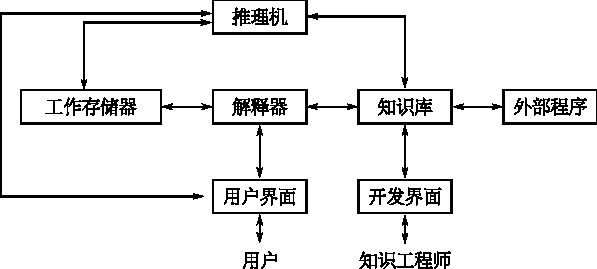
\includegraphics{figures/ans-6.6.pdf}
		\caption{基于规则的专家系统} \label{Fig:RES-structure}
	\end{figure}
基于规则的专家系统结构如图\ref{Fig:RES-structure}。主要由以下几部分组成:\par
	\begin{enumerate}
	\item 知识库。由谓词演算事实和有关讨论主题的规则构成。"知识工程师"与应用领域的专家共同工作以便把专家的相关知识表示成一种形式,由一个知识采集子系统协助,输入到知识库。\par
	\item 推理机。由所有操纵知识库来演绎用户要求的信息的过程构成——如消解、前向链或反向链。\par
	\item 用户界面。可能包括某种自然语言处理系统,它允许用户用一个有限的自然语言形式与系统交互。也可是用带有菜单的图形接口界面。\par
	\item 解释器。分析被系统执行的推理结构,并把它解释给用户。
	\item 开发界面。知识工程师通过该界面对专家系统进行开发。
	\item 工作存储器。建立人的短期存储器模型,存放问题事实和由规则激发而推断出的新事实。
	\item 外部程序。如数据库、扩展盘和算法等,对专家系统的工作起支持作用。它们应易于为专家系统所访问和使用。
	\end{enumerate}
\end{solution}

\begin{question}
什么是基于框架的专家系统?它与面向目标编程有何关系?
\end{question}
\begin{solution}
基于框架的专家系统采用了面向目标的编程技术,以提高系统的能力和灵活性。它们共享许多特征。\par
面向目标的编程其所有数据结构均以目标形式出现,每个目标含有两种基本信息:描述目标的信息和说明目标能做什么的信息。面向目标的编程为表示实际世界目标提供了一种自然的方法。\par
应用专家系统的术语来说,每个目标具有陈述性知识和过程知识。 
\end{solution}

\begin{question}
基于框架的专家系统的结构有何特点?其设计任务是什么?
\end{question}
\begin{solution}
基于框架的专家系统结构的主要特点在于基于框架的专家系统采用框架而不是规则来表示知识。框架提供一种比规则更丰富的获取问题知识的方法,不仅提供某些目标的包描述,而且还规定了该目标如何工作。 
开发基于框架的专家系统的主要任务有:
	\begin{enumerate}
		\item 定义问题(对问题和结论的考察与综述);
		\item 分析领域(定义事物,事物特征,事件和框架结构);
		\item 定义类及其特征;
		\item 定义例及其框架结构;
		\item 确定模式匹配规则;
		\item 规定事物通信方法;
		\item 设计系统界面;
		\item 对系统进行评价;
		\item 对系统进行扩展,深化和扩宽知识。
	\end{enumerate}
\end{solution}

\begin{question}
为什么要提出基于模型的专家系统?试述神经网络专家系统的一般结构。
\end{question}
\begin{solution}
有一种关于人工智能的观点认为:人工智能是对各种定性模型的获得、表达及使用的计算方法进行研究的学问。根据这一观点,一个知识系统中的知识库是由各种模型综合而成的,而这些模型又往往是定性的模型。 \par
采用各种定性模型来设计专家系统,一方面它增加了系统的功能,提高了性能指标,另一方面,可独立地深入研究各种模型及其相关问题,把获得的结果用于改进系统设计。
神经网络专家系统的一般结构如图\ref{Fig:NNES-structure}。
	\begin{figure}[h]
		\centering
		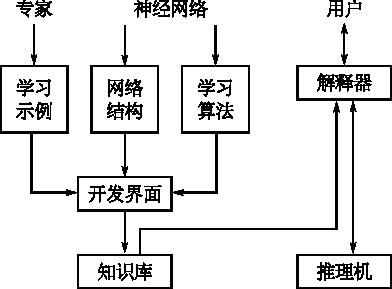
\includegraphics{figures/ans-6.7.pdf}
		\caption{神经网络专家系统} \label{Fig:NNES-structure}
	\end{figure}
\end{solution}

\begin{question}
为什么要提出基于Web的专家系统?试述基于Web的专家系统的一般结构。
\end{question}
\begin{solution}
随着互联网技术的发展,Web逐步成为大多数软件用户的交互接口,软件逐步走向网络化,体现为Web服务。因此专家系统的发展也离不开这个趋势,专家系统的用户界面已经逐步向Web靠拢,专家系统的知识库和推理机也都逐步与Web借口交互起来。\par 
基于Web的专家系统的结构将人机交互定位在Internet层次,专家、知识工程师和普通用户通过浏览器可访问专家系统应用服务器,将问题传递给Web推理机,然后Web推理机通过后台数据库服务器对数据库和知识库进行存取,来推导出一些结论,然后将这些结论告诉用户。由此,基于Web专家系统的结构主要分为3个层次:浏览器、应用逻辑层和数据库层。
\end{solution}

\begin{question}
举例介绍一个基于Web的专家系统。
\end{question}
\begin{solution}
基于Web的专家系统的一个例子是基于Web的拖网绞机专家系统。该系统采用C/S的网络结构模型,从总体功能来看,个客户端都只能完成整个拖网绞机专家系统的部分功能,各客户端之间相互协同工作起来完成全局的系统设计。在该系统中,Web服务器处于核心地位,协作任务的协调、管理和技术支持。而客户端通过网络与服务器连接,即可了解最新的设计信息,向服务器传递自己的成果,参加各种非实时的协作;客户端也可利用透明设计平台进行客户端之间的并行协作设计。
\end{solution}

\begin{question}
新型专家系统有何特征?什么是分布式专家系统和协同式专家系统? 
\end{question}
\begin{solution}
新型专家系统有以下一些特征:
	\begin{enumerate}
		\item 并行与分布处理
		\item 多专家系统协同工作
		\item 高级语言和知识语言描述 \par
		知识工程师只需用一种高级专家系统描述语言对系统进行功能、性能及接口描述,并用知识表示语言描述领域知识,专家系统生成系统就能自动或半自动地生生所需的专家系统。
		\item 具有自学习功能 \par
		具有高级的知识获取与学习功能 
		\item 引入新的推理机制 \par
		除了能进行演绎推理之外,还有归纳推理(联想、类比)、非标准逻辑推理(非单调逻辑推理、加权逻辑推理)及各种基于不完全知识和模糊知识的推理。
		\item 具有自纠错和自完善能力 
		\item 进的智能人机接口 \par
		理解自然语言,实现语声、文字、图形和图像的直接输入输出是如今人们对智能计算机提出的要求。 
	\end{enumerate}
	\begin{description}
		\item[分布式专家系统]
		具有分布处理的特征,能把一个专家系统的功能经分解以后分布到多个处理器上去并行地工作,从而有总体上提高系统的处理效率。它可以工作在紧耦合的多处理器系统环境中,也可工作在松耦合的计算机网络环境中,其总体结构在很大程度上依赖于其所在的硬件环境。 
		\item[协同式专家系统]
		又称为“群专家系统”,是一个能综合若干个相近领域或一个领域的多个方面的子专家系统互相协作,共同解决一个更广领域问题的专家系统。是克服一般专家系统的局限性的重要途径。它不着重于处理的分布和知识的分布,而是更强调子系统间的协同合作。它并不一定要求有多个处理机的硬件环境,而且一般都是在同一个处理机上实现各子专家系统的。
	\end{description}
\end{solution}

\begin{question}
在设计专家系统时,应考虑哪些技术?
\end{question}
\begin{solution}
在设计专家系统时应考虑如下技术:
	\begin{enumerate}
		\item 具有可靠知识与数据的小搜索空间问题 \par
		数据可靠(无噪声、无错误、不丢失、不多余)和知识可靠(不出现假的、近似的或推测性的结论),决定了系统具有单调性并可采用单路推理路线。而小搜索空间的问题一般允许采用穷举搜索策略。 
		\item 不可靠的数据或知识 \par
		这种情况应采用概率推理、模糊推理、不可靠数据的精确推理方法或专门的不确定性推理技术。
		\item 时变数据 \par
		一般要涉及时间推理技术,推理过程要求较复杂的表示法。
		\item 大搜索空间的问题 \par
		一般要引入启发式搜索策略或采用分层体系结构,来降低求解过程的复杂程度。对大空间的问题通常还要根据具体问题的特征采取相应的对策。
	\end{enumerate}
\end{solution}

\begin{question}
什么是建造专家系统的工具?你知道哪些专家系统工具,各有什么特点?
\end{question}
\begin{solution}
专家系统开发工具是一些比较通用的工具,作为设计和开发专家系统的辅助手段和环境,以求提高专家系统的开发效率、质量和自动化水平。专家系统工具是一种更高级的计算机程序设计语言。比一般的计算机高级语言具有更强的功能。 
主要分为骨架型工具(又称外壳)、语言型工具、构造辅助工具和支撑环境等4类。
	\begin{enumerate}
		\item 骨架型工具 \par
		借用以前开发好的专家系统,将描述领域知识的规则从原系统中"挖掉",只保留其独立于问题领域知识的推理机部分,这样形成的工具称为骨架型工具,如EMYCIN、KAS以及EXPERT等。\par
		其控制策略是预先给定的,使用起来很方便,用户只须将具体领域的知识明确地表示成为一些规则就可以了。这样,可以把主要精力放在具体概念和规则的整理上,从而大大提高了专家系统的开发效率。\par
		因其程序的主要骨架是固定的,除了规则以外,用户不可改变任何东西。使得骨架型工具的应用范围很窄,只能用来解决与原系统相类似的问题。
		\item 语言型工具 \par
		提供给用户的是建立专家系统所需要的基本机制,其控制策略也不固定于一种或几种形式,用户可以通过一定手段来影响其控制策略。因此,语言型工具的结构变化范围广泛,表示灵活,所适应的范围要比骨架型工具广泛得多。像OPS5、OPS83、RLL及ROSIE等,均属于这一类工具。\par
		使用起来比较困难,用户不易掌握,对于具体领域知识的表示也比骨架型工具困难一些,而且在与用户的对话方面和对结果的解释方面也往往不如骨架型工具。 
		\item 构造辅助工具 \par
		主要分2类,一类是设计辅助工具,典型的有AGE系统,另一类是知识获取辅助工具,典型的有TEIRESIAS系统。
 		\item 支撑环境 \par
		是指帮助进行程序设计的工具,它常被作为知识工程语言的一部分。工具支撑环境仅是一个附带的软件包,以便使用户界面更友好,它包括四个典型组件:调试辅助工具、输入输出设施、解释设施和知识库编辑器。ART就属于这一类系统。
	\end{enumerate}
\end{solution}

\begin{question}
专家系统面临什么问题?你认为应如何发展专家系统?
\end{question}
\begin{solution}
专家系统主要面临的问题包括以下几个方面:在体系结构上,目前大部分是单一的或独立的专家系统,所能解决问题的范围较窄;在知识获取方面,缺乏知识获取的能力;在问题求解方面,强调利用领域专家的经验性知识求解问题,忽视了深层知识在问题求解中的作用;在知识表示方法上缺少多种表示模式的集成,所能表示的知识面比较窄;在推理方面,不支持多种推理策略,缺少时态推理和非单调推理等人类思维中最常用的推理策略。所有这些缺点都决定了必须对专家系统技术做进一步的研究,开发功能更加强大的新一代专家系统。
\end{solution}

\begin{question}
基于规则的推理系统证明下述推理的正确性: 
	\begin{align*}
	\text{已知} \quad	& \text{狗都会吠叫和咬人} \\
					& \text{任何动物吠叫时总是吵人的} \\
					& \text{猎犬是狗} \\
	\text{结论} \quad	& \text{猎犬是吵人的}
	\end{align*}
\end{question}
\begin{solution}
推理过程:事实库初始化,使用规则与事实库匹配,更新事实库,并标记所用规则。\par
事实:猎犬;利用规则3得到结论;再利用规则1得到结论;再利用规则2得到结论:总是吵人的。
\end{solution}